\documentclass{article}

% NeurIPS 2026 submission style. The default option is the main-track,
% double-blind submission format (line numbers and anonymized author block).
\usepackage{neurips_2026}

\usepackage[utf8]{inputenc}
\usepackage[T1]{fontenc}
\usepackage{hyperref}
\usepackage{url}
\usepackage{booktabs}
\usepackage{amsmath}
\usepackage{amssymb}
\usepackage{nicefrac}
\usepackage{microtype}
\usepackage{xcolor}
\usepackage{graphicx}
\usepackage{tikz}
\usetikzlibrary{arrows.meta,positioning,calc}

\title{Sparse Latent Dynamics for Financial Forecasting under Market Shifts}

\author{%
  Four-Person Project Team \\
  CSC413 Course Project Proposal \\
  \texttt{Names and student IDs to be added}
}


\begin{document}
\maketitle

\begin{abstract}
Financial returns are noisy and nonstationary, making it difficult for sequence models to generalize across market conditions. We propose to test whether sparse latent dynamics improve next-day ETF return forecasting relative to a standard gated recurrent unit (GRU). A GRU encodes a fixed historical window into a low-dimensional state; a learned state transition is regularized using a small polynomial library and a sparsity penalty. We will compare a direct GRU, a dense latent-transition model, and a sparse latent-transition model using chronological out-of-sample evaluation on four liquid ETFs. Performance will be assessed with forecast errors and regime-stratified diagnostics. We will also examine whether discovered terms remain stable when the encoder is held fixed. The primary contribution is a controlled evaluation of a dynamical inductive bias, not a claim to discover universal financial laws. Regime-conditioned transitions and more elaborate rolling retraining are optional extensions.
\end{abstract}

\section{Introduction}
Financial return predictability can change as volatility, monetary conditions, and cross-asset relationships evolve. Recurrent neural networks can learn nonlinear patterns from sequential observations, but may overfit historical relationships. Sparse identification of nonlinear dynamics (SINDy) offers a complementary structural assumption: a low-dimensional state transition may be approximated by a small number of candidate terms \citep{brunton2016}.

Our question is: \emph{Does a sparse latent-state transition improve out-of-sample financial forecasting relative to an otherwise comparable GRU, particularly during volatile market periods?} We do not assume that prices obey a deterministic ordinary differential equation. Instead, we test whether a parsimonious approximate transition is a useful predictive inductive bias.

\paragraph{Input and output.}
For trading day $t$, the input is a lookback window $X_t=[x_{t-L+1},\ldots,x_t]\in\mathbb{R}^{L\times d_x}$ of historical features observed by the end of day $t$, with $L=40$ initially. The output is a vector $\hat y_{t+1}\in\mathbb{R}^{N}$ predicting next-day close-to-close log returns for $N=4$ ETFs. The prediction time is after the close on day $t$; any feature not available by then is excluded.

\paragraph{Planned contributions.}
\begin{enumerate}
\item A reproducible chronological evaluation of GRU forecasting on a small multi-asset panel.
\item A controlled comparison of direct GRU, dense latent transition, and sparse latent transition, using the same sequence encoder where possible.
\item An analysis of forecast errors in calm versus stressed markets and of sparse-term stability in a fixed latent coordinate system.
\end{enumerate}

\section{Background and Related Work}
\paragraph{Financial sequence models.}
Fischer and Krauss \citep{fischer2018} evaluate LSTM models for financial prediction, motivating recurrent encoders for historical return sequences. Our study uses a GRU and emphasizes controlled comparisons rather than a more complex predictive architecture.

\paragraph{Sparse dynamics discovery.}
SINDy \citep{brunton2016} represents state changes using a sparse combination of candidate nonlinear terms. Champion et al.\ \citep{champion2019} jointly learn latent coordinates and governing equations with an autoencoder. SINDy-SHRED \citep{gao2026sindyshred} combines recurrent representations with sparse latent dynamics. Thus, combining recurrent learning and SINDy is \emph{not} claimed as a new general method; we examine its usefulness for nonstationary financial prediction.

\paragraph{Nonstationarity and alternative dynamics.}
Wang and Lera \citep{wang2026} study return prediction under shifting market regimes. Nguyen et al.\ \citep{nguyen2024} investigate neural ODEs for stock forecasting. Unlike a neural-ODE approach, our core method uses a one-day discrete transition and does not require a numerical ODE solver. We focus on whether sparsity provides benefits beyond adding a transition layer.

\section{Data}
\paragraph{Assets and period.}
We plan to retrieve adjusted daily prices and volumes for SPY, QQQ, TLT, and GLD, provisionally covering 2010--2025, from a public market-data provider. The exact dates, missing observations, and data source will be documented after retrieval. The four ETFs represent overlapping equity exposures and distinct bond/gold exposures while keeping the dataset manageable.

\paragraph{Features and targets.}
For each ETF, candidate features include one-day log returns, trailing realized volatility, trailing momentum, and relative trading volume. All rolling features use observations available at or before $t$. The target for asset $i$ is
\begin{equation}
y_{t+1}^{(i)}=\log P_{t+1}^{(i)}-\log P_t^{(i)}.
\end{equation}
We will fit scaling and any clipping thresholds on training data only. Missing-data handling and the adjusted-price convention will be documented.

\paragraph{Chronological evaluation.}
We propose training on 2010--2019, validation on 2020--2021, and a held-out test on 2022--2025. Validation will determine hyperparameters; test results will be inspected only after model selection. We will evaluate stressed versus calmer days using a simple, predeclared market-volatility indicator computed from historical data. Such strata are for analysis, not inputs to a learned regime classifier. An additional rolling-origin experiment may be conducted if time permits.

\paragraph{Exploratory analysis.}
We will visualize return distributions, volatility clustering, and the contrast between calm and stressed periods. Figure~\ref{fig:vix} is an illustrative market-volatility diagnostic from the original exploratory analysis; the final dataset analysis will be recomputed for the chosen period and assets.

\begin{figure}[t]
  \centering
  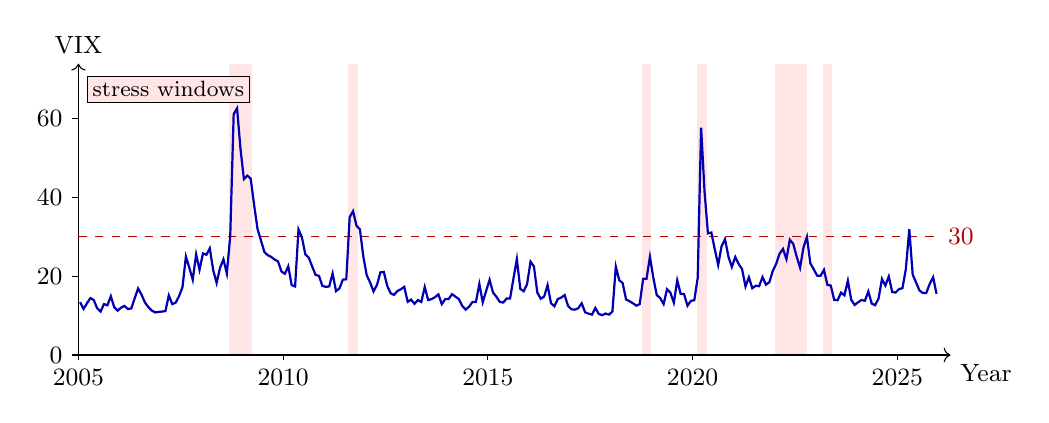
\begin{tikzpicture}[x=0.52cm,y=0.05cm,font=\small]
    % Shaded event windows are used only for evaluation.
    \fill[red!10] (3.67,0) rectangle (4.25,74);
    \fill[red!10] (6.59,0) rectangle (6.82,74);
    \fill[red!10] (13.76,0) rectangle (13.99,74);
    \fill[red!10] (15.10,0) rectangle (15.34,74);
    \fill[red!10] (17.02,0) rectangle (17.80,74);
    \fill[red!10] (18.19,0) rectangle (18.40,74);

    \draw[->] (0,0) -- (21.3,0) node[below right] {Year};
    \draw[->] (0,0) -- (0,74) node[above] {VIX};
    \foreach \y in {0,20,40,60} \draw (0,\y) -- (-0.15,\y) node[left] {\y};
    \foreach \x/\yr in {0/2005,5/2010,10/2015,15/2020,20/2025}
      \draw (\x,0) -- (\x,-1.3) node[below] {\yr};
    \draw[dashed, red!70!black] (0,30) -- (21.0,30) node[right] {30};
      \draw[blue!70!black, thick] plot coordinates { (0.042,13.44) (0.125,11.71) (0.208,13.13) (0.292,14.46)
     (0.375,13.97) (0.458,11.87) (0.542,11.05) (0.625,12.95) (0.708,12.63) (0.792,14.94) (0.875,12.15)
     (0.958,11.26) (1.042,12.04) (1.125,12.47) (1.208,11.69) (1.292,11.85) (1.375,14.45) (1.458,16.92)
     (1.542,15.33) (1.625,13.35) (1.708,12.18) (1.792,11.31) (1.875,10.82) (1.958,10.96) (2.042,11.04)
     (2.125,11.16) (2.208,15.16) (2.292,12.93) (2.375,13.30) (2.458,14.95) (2.542,17.27) (2.625,25.03)
     (2.708,22.20) (2.792,19.12) (2.875,25.58) (2.958,21.65) (3.042,25.82) (3.125,25.46) (3.208,27.10)
     (3.292,21.56) (3.375,18.30) (3.458,22.11) (3.542,24.32) (3.625,20.70) (3.708,30.24) (3.792,61.18)
     (3.875,62.67) (3.958,52.41) (4.042,44.68) (4.125,45.57) (4.208,44.80) (4.292,38.06) (4.375,31.98)
     (4.458,29.14) (4.542,26.16) (4.625,25.34) (4.708,24.93) (4.792,24.25) (4.875,23.79) (4.958,21.24)
     (5.042,20.64) (5.125,22.54) (5.208,17.77) (5.292,17.42) (5.375,31.93) (5.458,29.92) (5.542,25.57)
     (5.625,24.75) (5.708,22.52) (5.792,20.37) (5.875,20.10) (5.958,17.57) (6.042,17.32) (6.125,17.43)
     (6.208,20.72) (6.292,16.24) (6.375,16.91) (6.458,19.15) (6.542,19.23) (6.625,35.03) (6.708,36.53)
     (6.792,32.83) (6.875,31.94) (6.958,25.05) (7.042,20.23) (7.125,18.42) (7.208,16.17) (7.292,17.82)
     (7.375,21.00) (7.458,21.13) (7.542,17.57) (7.625,15.69) (7.708,15.28) (7.792,16.28) (7.875,16.70)
     (7.958,17.31) (8.042,13.51) (8.125,14.07) (8.208,13.03) (8.292,13.97) (8.375,13.49) (8.458,17.27)
     (8.542,13.97) (8.625,14.21) (8.708,14.69) (8.792,15.41) (8.875,12.92) (8.958,14.19) (9.042,14.24)
     (9.125,15.47) (9.208,14.84) (9.292,14.20) (9.375,12.48) (9.458,11.54) (9.542,12.30) (9.625,13.49)
     (9.708,13.47) (9.792,18.06) (9.875,13.41) (9.958,16.29) (10.042,19.12) (10.125,15.90) (10.208,14.81)
     (10.292,13.49) (10.375,13.34) (10.458,14.34) (10.542,14.35) (10.625,19.43) (10.708,24.38) (10.792,16.79)
     (10.875,16.21) (10.958,18.03) (11.042,23.72) (11.125,22.52) (11.208,15.85) (11.292,14.30) (11.375,14.85)
     (11.458,17.77) (11.542,13.16) (11.625,12.40) (11.708,14.22) (11.792,14.59) (11.875,15.24) (11.958,12.47)
     (12.042,11.61) (12.125,11.53) (12.208,11.90) (12.292,13.14) (12.375,10.86) (12.458,10.51) (12.542,10.26)
     (12.625,11.98) (12.708,10.44) (12.792,10.13) (12.875,10.54) (12.958,10.26) (13.042,11.06) (13.125,22.46)
     (13.208,19.02) (13.292,18.27) (13.375,14.12) (13.458,13.68) (13.542,13.15) (13.625,12.55) (13.708,12.91)
     (13.792,19.35) (13.875,19.39) (13.958,24.95) (14.042,19.57) (14.125,15.23) (14.208,14.49) (14.292,12.95)
     (14.375,16.72) (14.458,15.84) (14.542,13.31) (14.625,18.98) (14.708,15.56) (14.792,15.47) (14.875,12.52)
     (14.958,13.76) (15.042,13.94) (15.125,19.63) (15.208,57.74) (15.292,41.45) (15.375,30.90) (15.458,31.12)
     (15.542,26.84) (15.625,22.89) (15.708,27.65) (15.792,29.44) (15.875,25.00) (15.958,22.37) (16.042,24.91)
     (16.125,23.14) (16.208,21.84) (16.292,17.42) (16.375,19.76) (16.458,16.96) (16.542,17.60) (16.625,17.47)
     (16.708,19.82) (16.792,17.87) (16.875,18.50) (16.958,21.35) (17.042,23.18) (17.125,25.75) (17.208,26.97)
     (17.292,24.37) (17.375,29.31) (17.458,28.23) (17.542,25.00) (17.625,22.17) (17.708,27.34) (17.792,30.01)
     (17.875,23.30) (17.958,21.78) (18.042,20.17) (18.125,20.12) (18.208,21.64) (18.292,17.82) (18.375,17.64)
     (18.458,14.00) (18.542,13.93) (18.625,15.85) (18.708,15.17) (18.792,18.89) (18.875,14.02) (18.958,12.72)
     (19.042,13.39) (19.125,13.98) (19.208,13.79) (19.292,16.14) (19.375,13.06) (19.458,12.67) (19.542,14.37)
     (19.625,19.31) (19.708,17.66) (19.792,19.96) (19.875,16.02) (19.958,15.87) (20.042,16.76) (20.125,16.97)
     (20.208,21.84) (20.292,31.97) (20.375,20.46) (20.458,18.40) (20.542,16.38) (20.625,15.75) (20.708,15.79)
     (20.792,18.09) (20.875,19.77) (20.958,15.55) };
    \node[draw, fill=red!10, inner sep=2pt, font=\footnotesize, anchor=north west] at (0.2,71) {stress windows};
  \end{tikzpicture}
  \caption{Monthly average CBOE VIX over the proposed sample (FRED series VIXCLS, January 2005--December 2025). Shaded bands mark the stress windows used in the evaluation: the global financial crisis, the 2011 euro-area debt stress, 2018 Q4, the COVID-19 shock, the 2022 inflation and rate shock, and the 2023 regional-banking stress. The figure illustrates volatility clustering and abrupt regime changes; the stress labels are used only for evaluation and are never provided to the model.}
  \label{fig:vix}
\end{figure}

\section{Model Architecture}
\paragraph{Shared GRU encoder.}
A one-layer GRU with 64 hidden units maps each input window to a latent state:
\begin{equation}
z_t=E_\theta(X_t)\in\mathbb{R}^{m},\qquad m=4.
\end{equation}
The same input features and encoder configuration will be used across learned baselines.

\paragraph{Three principal models.}
The \emph{direct GRU} predicts $\hat y_{t+1}=h_\psi(z_t)$. The \emph{dense-transition GRU} uses
$\hat z_{t+1}=z_t+F_\phi(z_t)$ with a small MLP $F_\phi$, followed by $\hat y_{t+1}=h_\psi(\hat z_{t+1})$. The \emph{sparse-transition GRU} instead uses
\begin{equation}
\hat z_{t+1}=z_t+\Theta(z_t)\Xi,\qquad
\hat y_{t+1}=h_\psi(\hat z_{t+1}),
\end{equation}
where $\Theta(z_t)$ contains constant, linear, and quadratic monomials and $\Xi$ is a trainable coefficient matrix. All models predict next-day returns; only the transition model differs.

\paragraph{Objective and identifiability.}
The sparse model minimizes
\begin{equation}
\mathcal L=\mathcal L_{\rm pred}
+\lambda_d\|E_\theta(X_{t+1})-\hat z_{t+1}\|_2^2
+\lambda_s\|\Xi\|_1
+\lambda_r\mathcal L_{\rm rec}.
\end{equation}
Here $\mathcal L_{\rm pred}$ is return MSE, and $\mathcal L_{\rm rec}$ is an optional lightweight reconstruction loss to discourage latent collapse. The dense-transition baseline uses the corresponding transition-consistency term but no sparse coefficient penalty. Since jointly learned latent coordinates are not unique, we will not directly compare coefficients from independently retrained encoders. For interpretability tests, we will freeze a common encoder and fit or evaluate transitions in that fixed coordinate system.

\paragraph{Implementation.}
We will use PyTorch, AdamW, early stopping on validation MSE, and a small validation-selected grid of $\lambda_d$ and $\lambda_s$. Initial settings are a 40-day window, 64 GRU hidden units, latent dimension four, and batch size 64; these may be adjusted using validation data. Neural ODEs and regime-specific coefficient mixtures are not required for the core project and would be attempted only with instructor approval and sufficient time.

\subsection{Architecture Figure}
Figure~\ref{fig:architecture} is an original diagram of the proposed core model.
\begin{figure}[t]
\centering
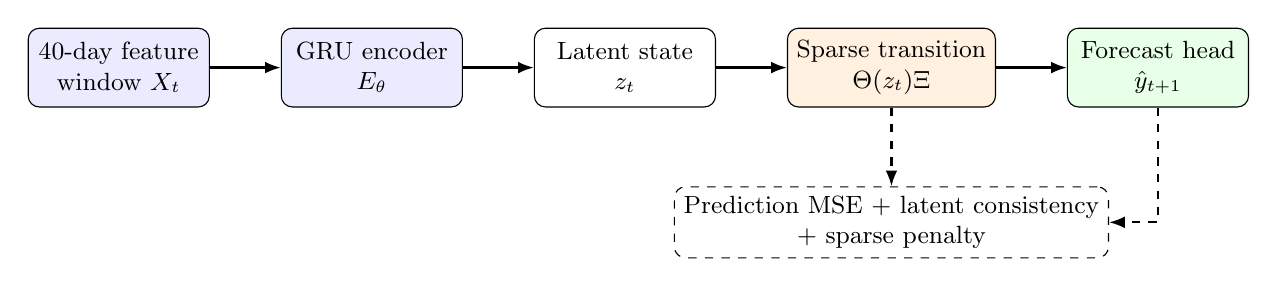
\begin{tikzpicture}[
  node distance=7mm and 9mm,
  every node/.style={font=\small},
  block/.style={draw,rounded corners,align=center,minimum height=10mm,minimum width=23mm},
  arr/.style={-{Latex[length=2mm]},thick}
]
\node[block,fill=blue!8] (x) {40-day feature\\window $X_t$};
\node[block,fill=blue!8,right=of x] (enc) {GRU encoder\\$E_\theta$};
\node[block,right=of enc] (z) {Latent state\\$z_t$};
\node[block,fill=orange!12,right=of z] (dyn) {Sparse transition\\$\Theta(z_t)\Xi$};
\node[block,fill=green!9,right=of dyn] (head) {Forecast head\\$\hat y_{t+1}$};
\draw[arr] (x)--(enc);
\draw[arr] (enc)--(z);
\draw[arr] (z)--(dyn);
\draw[arr] (dyn)--(head);
\node[draw,dashed,rounded corners,below=10mm of dyn,align=center] (loss) {Prediction MSE + latent consistency\\+ sparse penalty};
\draw[arr,dashed] (dyn)--(loss);
\draw[arr,dashed] (head.south) |- (loss.east);
\end{tikzpicture}
\caption{Original core architecture. The direct-GRU and dense-transition baselines replace the sparse transition while retaining the sequence input and forecast target.}
\label{fig:architecture}
\end{figure}

\section{Proposed Evaluation}
\paragraph{Baselines.}
We will report a zero-return predictor as a simple financial benchmark and compare three learned models: direct GRU, GRU with a dense latent transition, and GRU with a sparse latent transition. A generic weight-decay control will be included if resources permit.

\paragraph{Primary metrics.}
The main metrics are next-day return MSE, MAE, and directional accuracy. We will also report errors separately for predeclared calmer and stressed periods. All models will use identical chronological splits and feature availability assumptions.

\paragraph{Dynamics diagnostics.}
We will report the number of retained polynomial terms, one-step latent transition error, and whether active terms are stable across time blocks when using a frozen encoder. Because sparsity alone does not establish economic interpretability, we will describe discovered terms as model-dependent relationships rather than governing laws.

\paragraph{Reproducibility and optional extensions.}
We plan to run three seeds for the main models and report means and variability. If the core experiments finish early, we may add one rolling-origin refit, a transaction-cost-aware illustrative backtest, or regime-conditioned transition coefficients. These are explicitly secondary and will not be necessary to answer the primary question.

\section{Ethical Considerations}
Historical market prediction can be mistaken for investment advice. We will present results as a methodological comparison, not a deployable trading strategy. Retrospective tests may overstate usefulness due to data selection, transaction costs, and changing market conditions. We will report negative results and uncertainty, and avoid interpreting latent equations as causal or universal financial laws. Public-data licensing and reproducibility will be documented.

\section{Work Division}
The project will be completed by four students. The following provisional assignments will be confirmed by the team:
\begin{itemize}
\item \textbf{Member 1 (data and evaluation):} download and validate ETF data, implement chronological splits, prevent leakage, and prepare exploratory figures.
\item \textbf{Member 2 (sequence baselines):} implement the direct GRU and zero-return baseline, tune the GRU on validation data, and maintain reproducible training scripts.
\item \textbf{Member 3 (dynamics modeling):} implement dense and sparse latent transitions, consistency losses, and sparsity diagnostics.
\item \textbf{Member 4 (experiments and reporting):} coordinate model comparisons, regime-stratified evaluation, plots, and assembly of the proposal and final report.
\end{itemize}
All members will review experimental design, test integrated code, interpret results, and contribute to writing. We plan a weekly team meeting and a shared repository with documented responsibilities.

\begin{thebibliography}{9}
\small

\bibitem[Brunton et al.(2016)]{brunton2016}
S.~L. Brunton, J.~L. Proctor, and J.~N. Kutz.
\newblock Discovering governing equations from data by sparse identification of nonlinear dynamical systems.
\newblock \emph{Proceedings of the National Academy of Sciences}, 113(15):3932--3937, 2016.
\newblock DOI: 10.1073/pnas.1517384113.

\bibitem[Champion et al.(2019)]{champion2019}
K.~Champion, B.~Lusch, J.~N. Kutz, and S.~L. Brunton.
\newblock Data-driven discovery of coordinates and governing equations.
\newblock \emph{Proceedings of the National Academy of Sciences}, 116(45):22445--22451, 2019.
\newblock DOI: 10.1073/pnas.1906995116.

\bibitem[Gao et al.(2026)]{gao2026sindyshred}
M.~L. Gao, J.~P. Williams, and J.~N. Kutz.
\newblock Sparse identification of nonlinear dynamics and Koopman operators with Shallow Recurrent Decoder Networks.
\newblock \emph{Proceedings of the National Academy of Sciences}, 123(16):e2508144123, 2026.
\newblock DOI: 10.1073/pnas.2508144123.

\bibitem[Fischer and Krauss(2018)]{fischer2018}
T.~Fischer and C.~Krauss.
\newblock Deep learning with long short-term memory networks for financial market predictions.
\newblock \emph{European Journal of Operational Research}, 270(2):654--669, 2018.
\newblock DOI: 10.1016/j.ejor.2017.11.054.

\bibitem[Wang and Lera(2026)]{wang2026}
Y.~Wang and S.~C. Lera.
\newblock Meta-learning for return prediction in shifting market regimes.
\newblock \emph{Journal of Financial Markets}, 79:101042, 2026.
\newblock DOI: 10.1016/j.finmar.2025.101042.

\bibitem[Nguyen et al.(2024)]{nguyen2024}
A.~Q. Nguyen, S.~Ha, and H.~Thai.
\newblock Phase space reconstructed neural ordinary differential equations model for stock price forecasting.
\newblock In \emph{Proceedings of the Pacific Asia Conference on Information Systems (PACIS)}, 2024.

\end{thebibliography}

\end{document}
